\documentclass{article}

\usepackage{listings}
\usepackage{color}
\usepackage{hyperref}
\usepackage{float}
\usepackage[spanish]{babel}

\definecolor{dkgreen}{rgb}{0,0.6,0}
\definecolor{gray}{rgb}{0.5,0.5,0.5}
\definecolor{mauve}{rgb}{0.58,0,0.82}

\lstset{frame=tb,
  language=Python,
  aboveskip=3mm,
  belowskip=3mm,
  showstringspaces=false,
  columns=flexible,
  basicstyle={\small\ttfamily},
  numbers=none,
  numberstyle=\tiny\color{gray},
  keywordstyle=\color{blue},
  commentstyle=\color{dkgreen},
  stringstyle=\color{mauve},
  breaklines=true,
  breakatwhitespace=true
  tabsize=3
}




\usepackage[utf8]{inputenc}
\usepackage{verbatim}
\usepackage{parskip}

\addtolength{\textwidth}{4cm}
\addtolength{\hoffset}{-2cm}


\title{Tarea 3: No somos nada, hola Internet}
\author{ Manuel Figueroa\\
        201104513-0\\
  \texttt{manuel.figueroa@alumnos.usm.cl}
  \and
  Claudio Galaz\\
  201073598-2\\
  \texttt{claudio.galaz@alumnos.usm.cl}}
\date{20 de Junio de 2014}

\usepackage{natbib}
\usepackage{graphicx}

\begin{document}

\maketitle
\pagebreak

\section{Desarrollo}
\subsection{Usando Open Visual Traceroute}
Utilizando Open Visual Traceroute, escriba las direcciones y observe lo que sucede. Investigue y explique porque los paquetes toman las rutas que aparecen en la herramienta. ¿Cómo viajan los paquetes de un continente a otro? Liste los enlaces internacionales que tiene Chile para conectarse a Internet. 


Los routers y computadores del planeta no están conectados directamente, sino que forman una gran red de enlaces (cableadas) por todo el mundo, por ello, para enviar datos a una dirección que se encuentra alojada en algún lugar lejano es necesario pasar por distintos routers. Por ejemplo, en el caso de la solicitud de páginas web, es necesario pasar por un servidor que contiene la dirección IP a la cual está asignada el dominio solicitado, y ello lo resuelven unas bases de datos llamadas DNS, quienes pueden guardar muchas direcciones IP para un mismo nombre de dominio.

Para esta experiencia se usa Open Visual Traceroute, que consiste en un programa para realizar \textit{traceroute} con una interfaz gráfica cómoda para el usuario. El \textit{traceroute}, mediante el protocolo ICMP (Internet Control Message Protocol), sigue la ruta de un paquete a través de los distintos saltos que hace. Los \textbf{saltos} son los routers, computadores o cualquier cosa que se encuentre entre la fuente y el destino. 

Cada paquete tiene un campo llamado TTL (time to live), o tiempo de vida, que indica la cantidad de saltos que un paquete puede viajar antes de ser descartado, y el cual es seteado en la capa de aplicación. 

En cada salto, el número de TTL va disminuyendo en 1, y si el router de destino no es encontrado en ninguno de los saltos, el TTL se convierte en cero y el router bota el paquete, notificando al que envió originalmente. Típicamente el valor de TTL es 30.

Algunas consideraciones sobre el \textit{traceroute}:

\begin{itemize}
\item Solo se ve la dirección de los paquetes que están siendo enviados. Esto no quiere decir que los que sean enviados de vuelta usen la misma ruta. El tráfico podría ser enviado por otra red sin siquiera saberlo a menos que se haga un traceroute en ese sentido.

\item Lo que se ve identificado en el seguimiento es el puerto por el que los paquetes entraron al router. Nunca se es capaz de ver cuánto tráfico sale de ese router; sólo se puede ver cómo entra al router y luego cómo entra el siguiente paquete.

\item Existen maneras de identificar routers con su respectiva localización. Esta información puede resultar muy importante para identificar rutas con loops y ruteos poco óptimos.

\item A veces los paquetes del traceroute son bloqueados, lo que es debido a asuntos de seguridad o protección contra DDoS.

\end{itemize}

Entonces, analizando lo obtenido con el programa se puede observar que en la mayoría de los casos el paquete sale del país; sólo con http://moodle.inf.utfsm.cl el paquete se queda en Chile. Esto sucede porque la plataforma Moodle del departamento es frecuentemente solicitada dentro de Chile, entonces no hay necesidad de ir a buscar la dirección a un servidor DNS fuera del país porque ya está guardada en el caché del servidor nacional. Al final llega a Valparaíso puesto que el Moodle del departamento de informática se encuentra alojado en Casa Central. 

Para http://cime.cl es necesario ir a buscar la DNS a otro lugar fuera de Chile, y luego va a Estados Unidos, donde el mayor tiempo de DNS Lookup se ocupa en New York y además es donde probablemente esté alojado el sitio. Hay que destacar el hecho que de los cinco sitios analizados es el que más tiempo ocupa en el DNS lookup.

Con Google ocurre algo totalmente distinto. Al ser el sitio más solicitado en Chile\footnote{``Revelan mapa con los sitios más visitados por país: Google es el favorito en Chile.'' \url{http://goo.gl/vXLb9V}}, claramente el DNS lookup ocurre dentro de Chile, por lo que el paquete es enviado inmediatamente a los Estados Unidos que es donde se encuentra alojado. 

Con Wikipedia el paquete viaja hasta España, y luego es enviado a Francia dos veces, donde pasa una gran cantidad de tiempo en el DNS lookup, buscando por la dirección a la cual corresponde el nombre. Luego de eso pasa por un router en New York antes de llegar a San Francisco.

Por último con la embajada de Australia, luego de viajar varios kilómetros hacia España y además hacer saltos por Europa, el paquete llega a Japón, donde luego de 10 segundos (timeout seteado por defecto en la aplicación) no muestra ningún otro salto. Aunque con un poco de demora puesto que debe dar la vuelta completa al planeta para llegar a Australia (donde debería estar alojado el sitio), el sitio carga perfectamente, lo que se debe a que el router en Japón permite el tráfico HTTP pero no los paquetes del protocolo ICMP, a quienes los hace esperar indefinidamente o simplemente los desecha, causando timeout.

La evidencia con los screen shots se encuentra en la sección de Anexos.

Con respecto a cómo viajan los paquetes de un continente a otro, lo hacen mediante cables submarinos y en la actualidad existen tres enlaces internacionales de fibra óptica en Chile, los que sirven para comunicar a nuestro país con el resto del mundo. Aquellos cables son:
\begin{itemize}
\item Pan American (PanAm), en Arica, conectado con Perú, Ecuador, Panamá, Colombia, Venezuela y las Islas Virginias.
\item South America-1 (SAm-1), encontrado en Arica y Valparaíso, conectando la mayoría de los países de Sudamérica con América Central. Observar la figura en los anexos.
\item South American Crossing (SAC)/Latin American Nautilus (LAN), que se encuentra en Valparaíso y conecta a Perú, Colombia, Panamá, Venezuela, las Islas Virginias, Brasil y Argentina.
\end{itemize}
Hay que destacar que para Julio de 2016 estará listo el South America Pacific Link (SAPL), que se encontrará en Arica y Valparaíso, teniendo conexión con Oahu en Hawaii. Esto permitirá una transmisión de paquetes más ágil con el resto del mundo.

Imágenes de los enlaces anteriores pueden ser consultados en la sección Anexos.

En la actualidad el continente antártico es el único que no tiene conexión por cable con el resto del mundo, realizando todo tipo de comunicaciones vía satélite. Esto es debido al tipo de cable que es necesario desarrollar para soportar las temperaturas de Antártica. En la actualidad el tipo de cable submarino usado para conectar internet entre continentes se compone de (enlistados desde la capa más exterior y hacia el interior):

\begin{itemize}
\item Polietileno.
\item BoPET.
\item Alambres de acero trenzado.
\item Barrera de aluminio resistente al agua.
\item Policarbonato.
\item Tubo de cobre o aluminio.
\item Vaselina.
\item Fibras ópticas.
\end{itemize}

\begin{figure}[H]
    \centering
    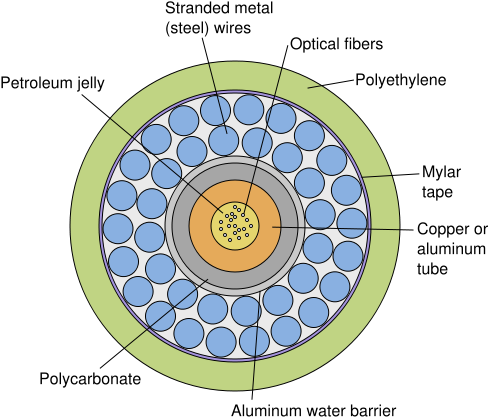
\includegraphics[scale=0.3]{cable}
    \caption{El cable submarino de comunicaciones y una mirada a través de un corte transversal}
\end{figure}

\subsection{Cálculo de rutas: Algoritmo vector-distancia}
Se dispone de la siguiente red a menor escala compuesta por 9 routers. El PC desea acceder a los archivos que se encuentran en el servidor.

\begin{figure}[H]
    \centering
    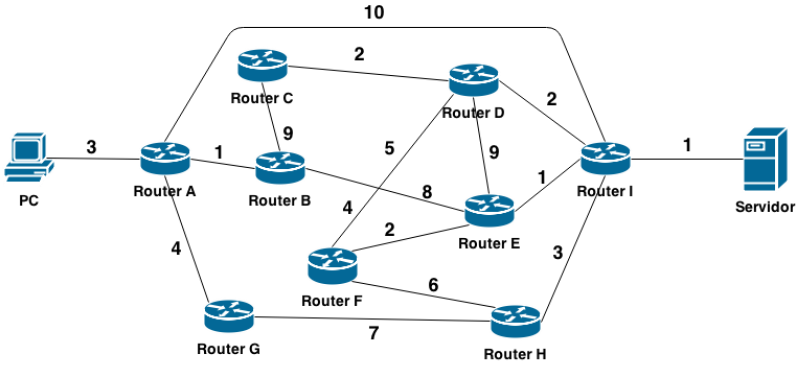
\includegraphics[scale=0.55]{grafo}
\end{figure}

Utilizando el Algoritmo Vector-Distancia, encuentre las tablas de costos de todos los routers.

En Python se realizó un script que aplica el algoritmo vector-distancia para encontrar las distancias mínimas entre nodos. El script imprime en consola las matrices que muestran la distancia entre los distintos con cada iteración.

\begin{figure}[H]
    \centering
    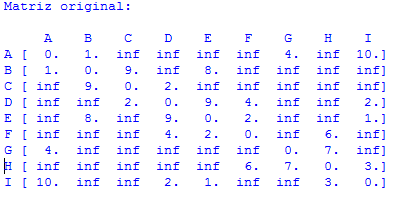
\includegraphics[scale=0.7]{original}
    \caption{Matriz de distancias original.}
\end{figure}

La matriz original muestra la distancia entre cada nodo y sus adyacentes, aquellos que no son adyacentes tienen un valor infinito. Es una forma simple de mostrar la matriz que tiene cada nodo, donde sólo poseen la información de las distancias entre ellos y sus adyacentes, es decir: su  vector fila con información y el resto en infinito.

Teniendo lo anterior en cuenta, para la primera iteración se asume que los nodos hicieron un broadcast de sus vectores distancia y todos los nodos poseen la matriz original. En base a esto se realiza el cálculo de las distancias mínimas de la siguiente forma:

\begin{center}
\begin{equation} \label{eq:1}
D_x(y) = min\{c(x,v)+D_v(y)\} 
\end{equation} 
\end{center}
para cada nodo y $\in$ N, siendo N el conjunto de los routers.

La función de distancia asigna el valor mínimo de la suma de la distancia a cada nodo vecino con la distancia entre éste y el nodo al que se quiere llegar. Cuando se actualizan las distancias, el algoritmo revisa si alguna distancia cambió, de ser así se realiza otra iteración hasta lograr llegar a los valores mínimos posibles.

La siguiente figura muestra las iteraciones sobre la matriz inicial:
\begin{figure}[H]
    \centering
    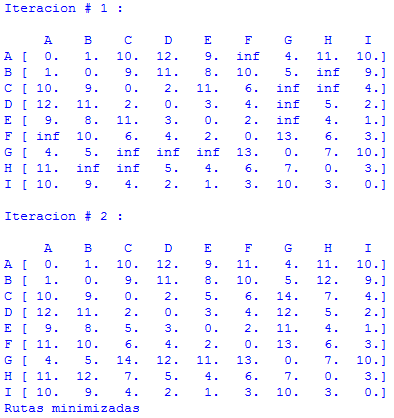
\includegraphics[scale=0.7]{rutas}
    \caption{Iteraciones para obtener distancias mínimas.}
\end{figure}
    
En tan sólo dos iteraciones se obtienen los valores mínimos de distancia entre nodos.


\subsection{Emergencia en la red}
Un barco transatlántico ha cortado el enlace entre los nodos H e I, ¿Cómo se comporta el algoritmo vector distancia en este caso? Recalcule solo los costos necesarios para resolver este problema.

Con una pequeña modificación al script anterior, se hace que cada vez que se utilice el enlace H-I en el cálculo de distancia entre dos nodos, se marque éste par de nodos.

\begin{figure}[H]
    \centering
    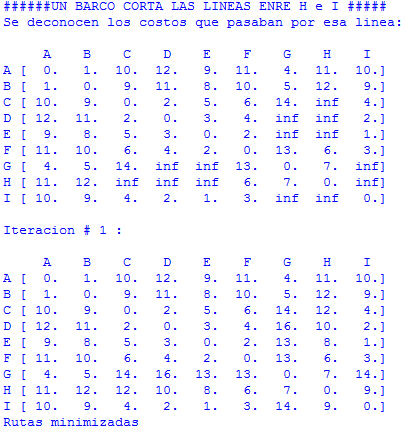
\includegraphics[scale=0.7]{post-barco}
    \caption{Iteraciones para obtener distancias luego del accidente.}
\end{figure}

Como se observa en la matriz de la figura 4, las distancias que fueron marcadas por usar el enlace H-I fueron cambiadas por ``Inf'', dado que sin el enlace disponible se desconoce la distancia mínima. Luego de esto se itera de nuevo para encontrar las distancias mínimas que se perdieron sin considerar dicho enlace.

    
\section{Referencias}
\begin{itemize}
\item Kurose, Jim. (2009). \textbf{Computer Networking: A Top Down Approach}, 5th Edition.
\item TeleGeography. \textbf{Submarine Cable Map} \url{http://www.submarinecablemap.com/}
\end{itemize}




\pagebreak
\section{Anexos}

\subsection{ejercicio 2.py}
El script genera todo lo necesario para las preguntas 2 y 3, obteniendo la distancia mínima entre los nodos y arreglando el error cuando se corta el enlace entre H e I.

\begin{lstlisting}
# -*- coding: cp1252 -*-
from numpy import *

def matriz_1():
    a = zeros((9,9))
    a[0] = [0,1,inf,inf,inf,inf,4,inf,10]
    a[1] = [1,0,9,inf,8,inf,inf,inf,inf]
    a[2] = [inf,9,0,2,inf,inf,inf,inf,inf]
    a[3] = [inf,inf,2,0,9,4,inf,inf,2]
    a[4] = [inf,8,inf,9,0,2,inf,inf,1]
    a[5] = [inf,inf,inf,4,2,0,inf,6,inf]
    a[6] = [4,inf,inf,inf,inf,inf,0,7,inf]
    a[7] = [inf,inf,inf,inf,inf,6,7,0,3]
    a[8] = [10,inf,inf,2,1,inf,inf,3,0]
    return a

def imprimir(a):
    bla = ['A','B','C','D','E','F','G','H','I']
    print "     A    B    C    D    E    F    G    H    I"
    for i in range(9):
        print bla[i], a[i]

def rutas(a,marcas):
    anterior = copy(a)
    contador = 0
    while True:
        contador += 1
        for i in range(9):
            for j in range(9):
                for z in range(9):
                    temp = copy(a[i,j])
                    a[i,j] = min(a[i,j], (anterior[i,z]+anterior[z,j]))
                    if (z == 7 and (i==8 or j==8)) or (z==8 and (i==7 or j==7)) or marcas[i,z]== 1 or marcas[z,j] ==1:
                        if temp != a[i,j]:
                            marcas[i,j] = 1
        if array_equal(a,anterior):
            print "Rutas minimizadas"
            break
        print "\nIteracion #",contador,":\n"
        imprimir(a)
        anterior = copy(a)
    return a

        
def main():
    a = matriz_1()
    marcas = zeros((9,9))
    print "Matriz original: \n"
    imprimir(a)
    rutas(a,marcas)
    print"\n######UN BARCO CORTA LAS LINEAS ENRE H e I #####"
    a[7,8] = float("inf")
    a[8,7] = float("inf")
    for m in range(9):
        for n in  range(9):
            if marcas[m,n] == 1:
                a[m,n]=float("inf")
    print "Se deconocen los costos que pasaban por esa linea:\n"
    imprimir(a)
    rutas(a, marcas)
    

if __name__ == '__main__':
    main()

\end{lstlisting}

\newpage
\subsection{Screenshots de Open Visual Traceroute}
Para una mayor resolución se puede consultar el directorio fuente del informe.
\begin{figure}[H]
    \centering
    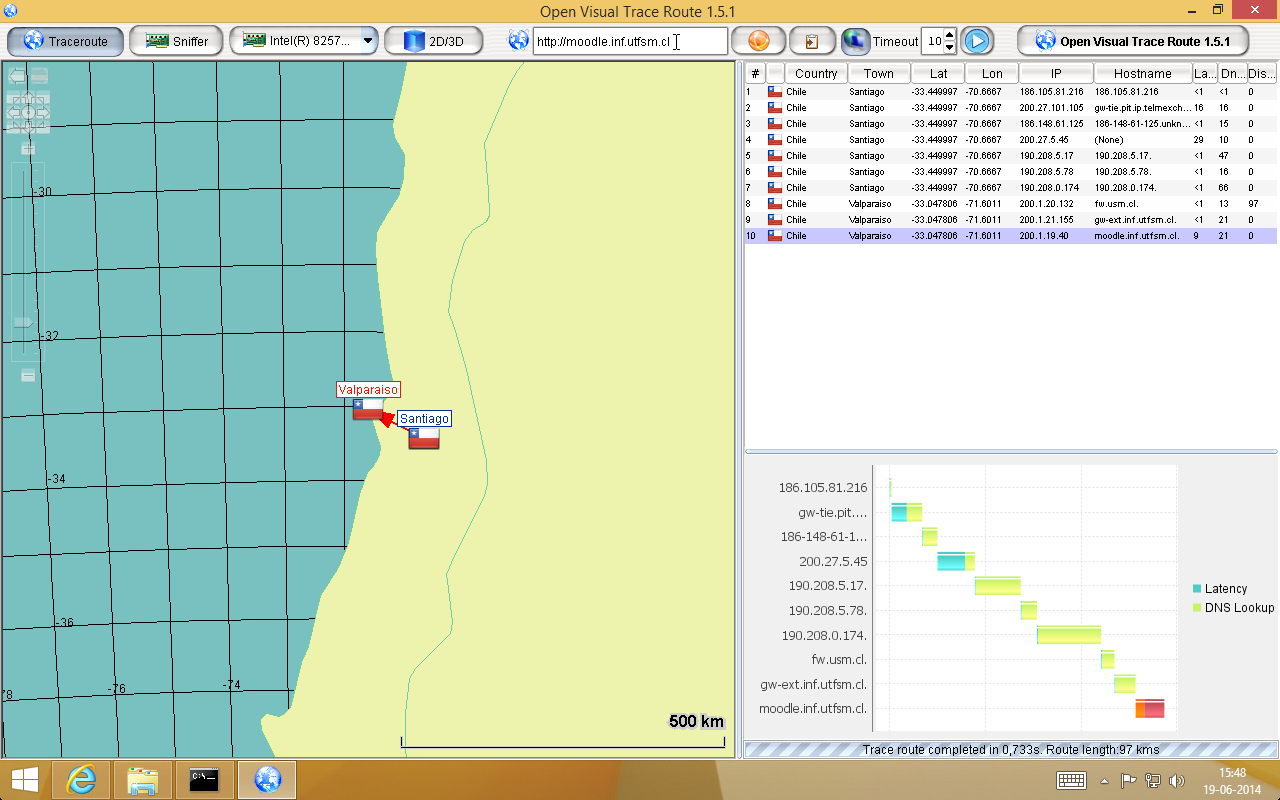
\includegraphics[scale=0.27]{mudul}
    \caption{Traceroute para el sitio http://moodle.inf.utfsm.cl}
\end{figure}

\begin{figure}[H]
    \centering
    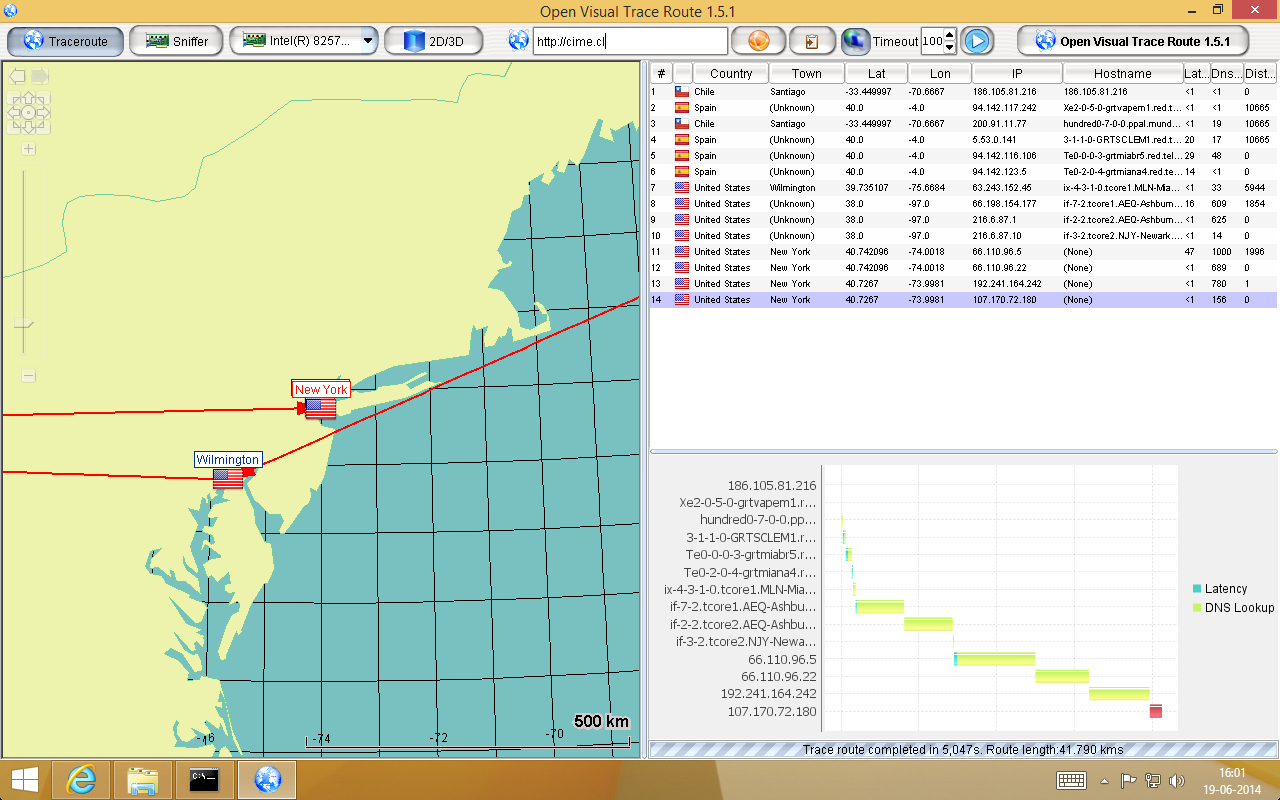
\includegraphics[scale=0.27]{cime}
    \caption{Traceroute para el sitio http://cime.cl}
\end{figure}

\begin{figure}[H]
    \centering
    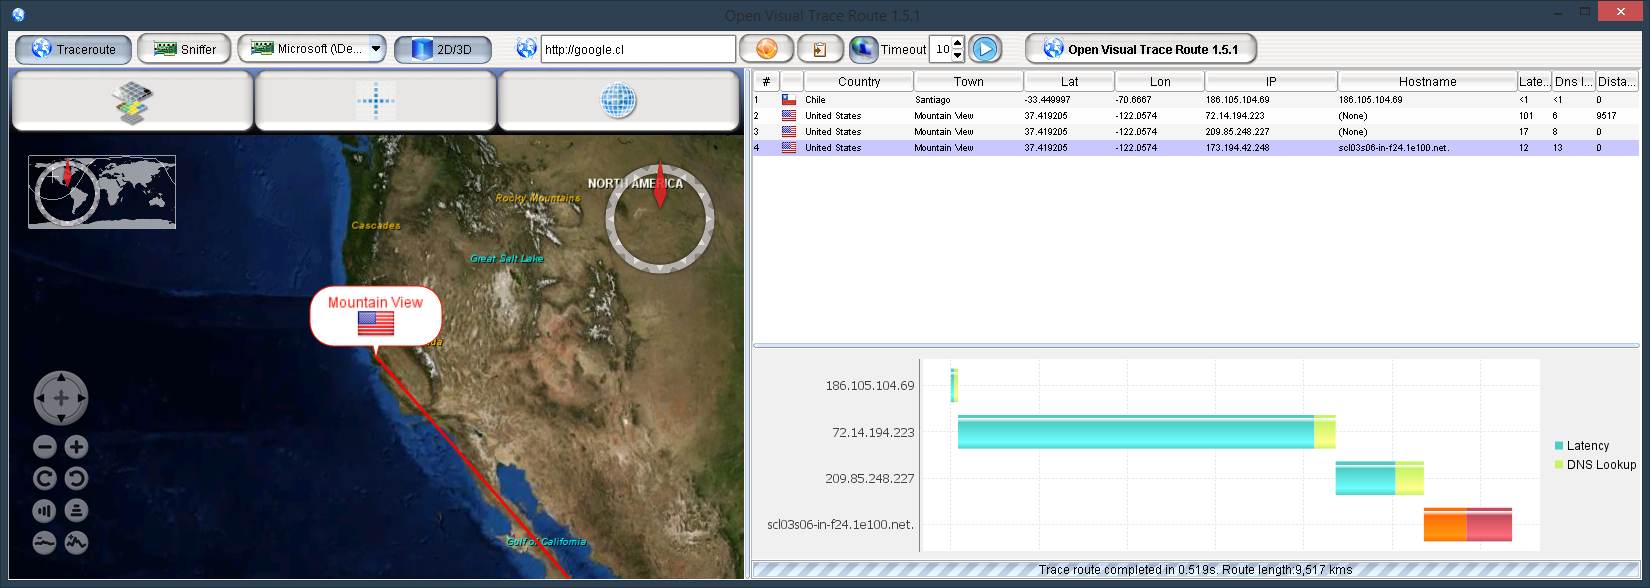
\includegraphics[scale=0.24]{gugl}
    \caption{Traceroute para el sitio http://google.cl}
\end{figure}

\begin{figure}[H]
    \centering
    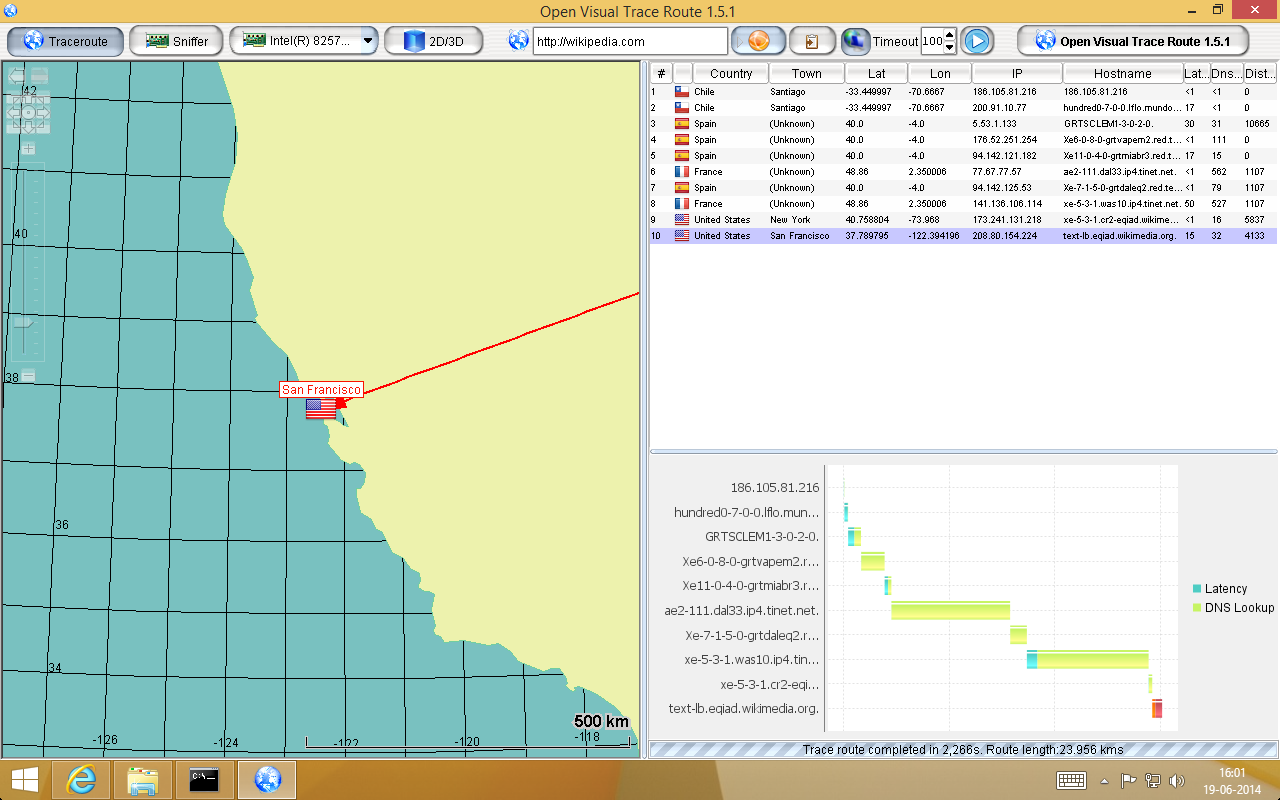
\includegraphics[scale=0.27]{wiki}
    \caption{Traceroute para el sitio http://wikipedia.com}
\end{figure}

\begin{figure}[H]
    \centering
    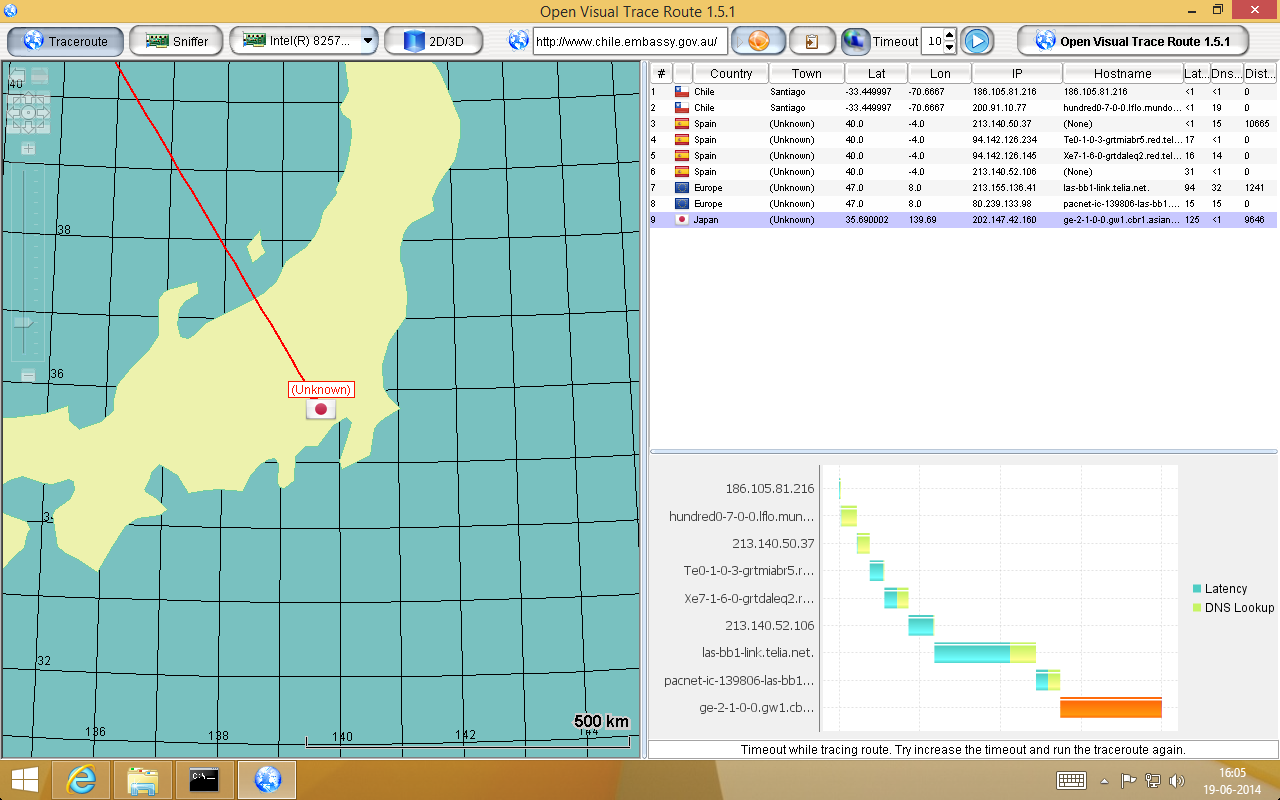
\includegraphics[scale=0.27]{embajada}
    \caption{Traceroute para el sitio http://www.chile.embassy.gov.au}
\end{figure}


%BLA
\subsection{Cables submarinos en enlace con Chile}

\begin{figure}[H]
    \centering
    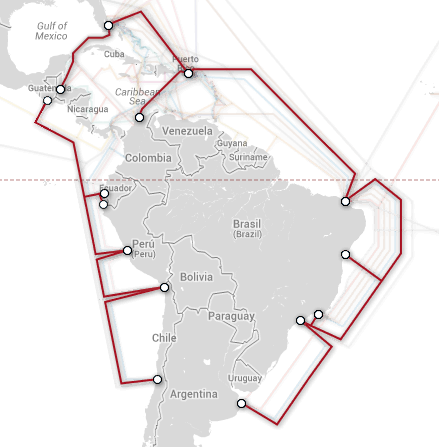
\includegraphics[scale=0.5]{SAm-1}
    \caption{Conexiones de South America-1}
\end{figure}

\begin{figure}[H]
    \centering
    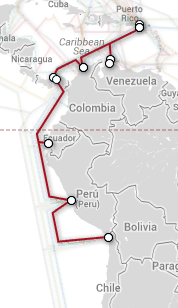
\includegraphics[scale=0.54]{PanAm}
    \caption{Conexiones de Pan American}
\end{figure}

\begin{figure}[H]
    \centering
    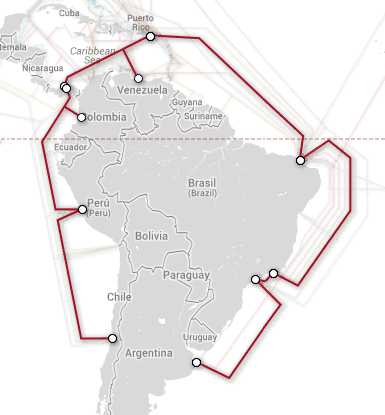
\includegraphics[scale=0.5]{SAC-LAN}
    \caption{Conexiones de South American Crossing/Latin American Nautilus}
\end{figure}

\begin{figure}[H]
    \centering
    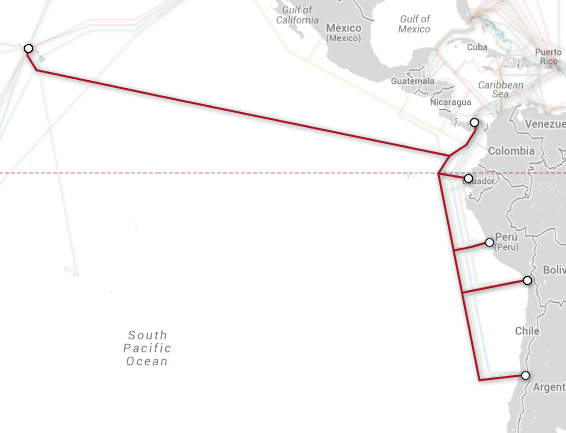
\includegraphics[scale=0.5]{SAmPL}
    \caption{Conexiones de South America Pacific Link (en proceso)}
\end{figure}



\end{document}
